%!TeX root=../tese.tex
%("dica" para o editor de texto: este arquivo é parte de um documento maior)
% para saber mais: https://tex.stackexchange.com/q/78101/183146

%% ------------------------------------------------------------------------- %%
\chapter{Interpretação geométrica de buscas em ABBs}
\label{cap:geometria}

Neste capítulo iremos entender como interpretar de maneira geométrica os algoritmos de busca em ABBs.

\section{Introdução}

Os algoritmos de busca dentro do modelo de computação adotado sempre iniciam o nó corrente na raiz da ABB e estrategicamente percorrem a árvore comparando a chave procurada com o nó corrente até encontrar o nó buscado.

Por simplicidade das provas, neste capítulo definiremos que todas as chaves são buscadas uma única vez, logo $n = m$.

Dada uma sequência $X = (x_{1},\ldots,x_{m})$ de $m$ acessos às chaves $x_{1}, x_{2},\ldots,x_{m}$, é possível ilustrar essas buscas de maneira gráfica.

Definindo um gráfico com o eixo X representando as chaves armazenadas dentro da ABB e com o eixo Y representando a buscas. Assim, o ponto na coordenada (p.x,p.y) representa que no instante de tempo p.y, a chave p.x foi buscada na ABB.

\begin{figure}
    \centering    
        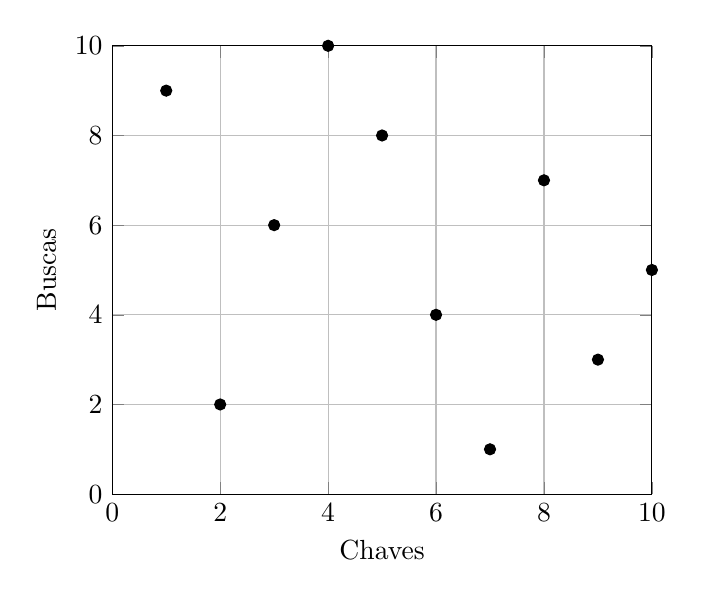
\begin{tikzpicture}
        \begin{axis}[
            xlabel={Chaves},
            ylabel={Buscas},
            grid=major,
            xmin=0, xmax=10,
            ymin=0, ymax=10,
            xtick={0,2,4,6,8,10},
            ytick={0,2,4,6,8,10}
        ]
        \addplot[only marks, mark=*] coordinates {
            (1,9)
            (2,2)
            (3,6)
            (4,10)
            (5,8)
            (6,4)
            (7,1)
            (8,7)
            (9,3)
            (10,5)
        };
        \end{axis}
        \end{tikzpicture}
    \caption{O gráfico representa a busca (7, 2, 9, 6, 10, 3, 8, 5, 1, 4)}
    \label{grafico2D-exemplo-inicial}
\end{figure}


\textit{Conjuntos arboreamente satisfeitos}: um par de pontos (a,b) do conjunto $P$ é arboreamente satisfeito se a e b são ortogonalmente colineares ou se há pelo menos um ponto do conjunto \( P \setminus \{a,b\} \) que está dentro da área delimitada pelo retângulo de vértices a e b. Um conjunto $P$ é arboreamente satisfeito se todos os pares de pontos do conjunto são arboreamente satisfeitos.

Em todo par de pontos (a,b) não ortogonalmente colineares, há sempre pelo menos um ponto de \( P \setminus \{a,b\} \) que está em alguma aresta que incide em a, e há também pelo menos um ponto que está em alguma aresta que incide em b.

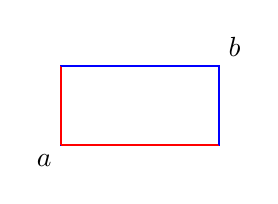
\begin{tikzpicture}
    % Desenha o retângulo
    \draw[blue, thick] (0,0) rectangle (2,1);
    
    % Adiciona os rótulos
    \node at (0,0) [below left] {$a$};
    \node at (2,1) [above right] {$b$};
    
    % Desenha as arestas de a para b
    \draw[red, thick] (0,0) -- (0,1);
    \draw[red, thick] (0,0) -- (2,0);
    \draw[blue, thick] (2,1) -- (0,1);
    \draw[blue, thick] (2,1) -- (2,0);
\end{tikzpicture}

Prova: 